\section{Capítulo 11 -- Introdução às estruturas de dados}

No fim do Capítulo 10, os dados de cada aluno estavam espalhados em dois vetores paralelos, e bastava esquecer de trocar um deles para os nomes se separarem das notas. O problema é de \textbf{organização}: os programas ficam mais simples e mais seguros quando os dados são guardados de uma forma que combina com o uso que se faz deles. Essa é a ideia de \textbf{estrutura de dados}. Neste capítulo você vai conhecer os \textbf{registros}, que reúnem dados diferentes sobre a mesma coisa, e três estruturas clássicas, cada uma com suas regras de entrada e saída: a \textbf{pilha}, a \textbf{fila} e a \textbf{lista encadeada}. Para construir a última, você também vai dar os primeiros passos com \textbf{ponteiros}.

\subsection{11.1 Registros}

Um \textbf{registro} reúne, sob um único nome, várias informações que podem ser de tipos diferentes. Cada informação é um \textbf{campo}. Um aluno tem nome (texto), matrícula (inteiro) e nota (real); em vez de três variáveis soltas, um registro \texttt{Aluno} guarda as três juntas. Em C++, um registro é declarado com \texttt{struct}, e os campos são acessados com um ponto:

\begin{codigo}
\begin{Verbatim}[breaklines=true, breaksymbolleft={}, fontsize=\footnotesize]
#include <iostream>
#include <string>
using namespace std;

struct Aluno {                 // um novo tipo, com três campos
    string nome;
    int matricula;
    double nota;
};

int main() {
    Aluno a;
    a.nome = "Ana";
    a.matricula = 2026001;
    a.nota = 8.5;
    Aluno b = {"Bruno", 2026002, 7.0};   // todos de uma vez
    cout << a.nome << " (" << a.matricula << "): " << a.nota
         << endl;                         // Ana (2026001): 8.5
    Aluno c = a;                          // copia tudo
    c.nota = 10;
    cout << a.nota << " " << c.nota << " " << b.nome << endl;
    return 0;                             // 8.5 10 Bruno
}
\end{Verbatim}
\end{codigo}

A declaração \texttt{struct Aluno} cria um \textbf{tipo novo}, que se usa como \texttt{int} ou \texttt{string}: dá para declarar variáveis, copiar com \texttt{=}, passar para funções e devolver com \texttt{return}. Como um registro pode ser grande, a passagem por referência constante (Capítulo 6) é a forma usual de entregá-lo a uma função que só vai lê-lo: \texttt{void mostrar(const Aluno \&a)}.

Na notação de Portugol usada em muitos livros, o registro é declarado com \texttt{tipo ... registro}. As ferramentas de Portugol variam no suporte a esse recurso, mas a ideia é a mesma:

\begin{codigo}
\begin{Verbatim}[breaklines=true, breaksymbolleft={}, fontsize=\footnotesize]
algoritmo "Registro"
tipo Aluno = registro
   nome: caractere
   matricula: inteiro
   nota: real
fimregistro
var
   a: Aluno
inicio
   a.nome <- "Ana"
   a.matricula <- 2026001
   a.nota <- 8.5
   escreval(a.nome, ": ", a.nota)
fimalgoritmo
\end{Verbatim}
\end{codigo}

\subsection{11.2 Vetores de registros}

Registros e vetores se combinam naturalmente: um vetor de \texttt{Aluno} é a turma inteira, e \texttt{turma[i].nota} é a nota do aluno \texttt{i}. Agora, ao ordenar, cada aluno se move \textbf{inteiro}, e o problema dos vetores paralelos desaparece. Melhor ainda: o \texttt{sort} da biblioteca aceita um terceiro argumento, uma função que diz se um elemento deve vir antes de outro, e assim ordena registros pelo critério que se quiser.

\begin{codigo}
\begin{Verbatim}[breaklines=true, breaksymbolleft={}, fontsize=\footnotesize]
#include <iostream>
#include <string>
#include <vector>
#include <algorithm>
using namespace std;

struct Aluno {
    string nome;
    double nota;
};

// a deve vir antes de b? Sim, se tiver nota maior.
bool maiorNota(const Aluno &a, const Aluno &b) {
    return a.nota > b.nota;
}

int main() {
    vector<Aluno> turma = {
        {"Ana", 7.5}, {"Bruno", 9.0}, {"Carla", 6.0},
        {"Diego", 9.5}, {"Elisa", 8.0}, {"Fabio", 5.5}
    };
    turma.push_back({"Gabi", 8.7});          // mais um cadastro
    sort(turma.begin(), turma.end(), maiorNota);
    for (size_t i = 0; i < turma.size(); i++) {
        cout << i + 1 << "o " << turma[i].nome << " ("
             << turma[i].nota << ")" << endl;
    }
    return 0;
}
// 1o Diego (9.5)  2o Bruno (9)  3o Gabi (8.7)  4o Elisa (8)
// 5o Ana (7.5)    6o Carla (6)  7o Fabio (5.5)
\end{Verbatim}
\end{codigo}

Compare com o programa da Seção 10.8: não há mais dois vetores para manter em sincronia, a ordenação é uma única linha, e acrescentar um campo novo, como a matrícula, não exige mudar a ordenação.

\subsection{11.3 Estruturas de dados e suas operações}

Uma \textbf{estrutura de dados} é uma forma de organizar dados na memória junto com as \textbf{operações} que se pode fazer sobre eles: inserir, remover, procurar, percorrer. O vetor é a mais simples: acesso direto a qualquer posição, mas inserir no meio exige deslocar todos os elementos seguintes. Cada estrutura faz algumas operações muito bem e outras mal, e escolher a estrutura certa é, muitas vezes, o que separa um programa rápido de um lento.

Ao estudar uma estrutura, vale separar duas perguntas. A primeira é \textbf{o que} ela faz: quais operações oferece e com que regras. A segunda é \textbf{como} ela faz: com vetores, com ponteiros, de que jeito. A descrição só da primeira parte é chamada de \textbf{tipo abstrato de dados}. Quem usa uma pilha precisa saber que o último a entrar é o primeiro a sair; não precisa saber se por dentro há um vetor. As próximas seções apresentam três tipos abstratos clássicos e uma forma simples de implementar cada um.

\subsection{11.4 Pilha}

Uma \textbf{pilha} funciona como uma pilha de pratos: um prato novo é colocado no topo, e o único que pode ser retirado é o do topo. O último a entrar é o primeiro a sair, regra conhecida pela sigla em inglês \textbf{LIFO} (\textit{last in, first out}). As operações são \textbf{empilhar} (\textit{push}), \textbf{desempilhar} (\textit{pop}), consultar o \textbf{topo} e verificar se a pilha está \textbf{vazia}.

\begin{center}
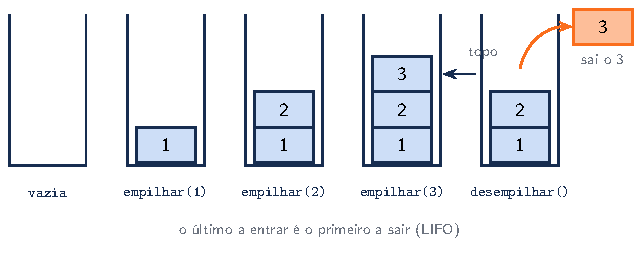
\includegraphics[width=0.85\linewidth,keepaspectratio]{imagens/capitulo-11_pilha.pdf}
\end{center}

Pilhas estão por toda parte na computação: o botão ``desfazer'' de um editor guarda as ações em uma pilha, o botão ``voltar'' do navegador guarda as páginas visitadas, e a pilha de chamadas do Capítulo 6 é, como o nome diz, uma pilha. A implementação mais simples usa um vetor e um contador, \texttt{topo}, que indica quantos elementos há (e, portanto, a próxima posição livre):

\begin{codigo}
\begin{Verbatim}[breaklines=true, breaksymbolleft={}, fontsize=\footnotesize]
#include <iostream>
#include <string>
using namespace std;

const int MAX = 100;

struct Pilha {
    char dados[MAX];
    int topo = 0;              // quantos elementos há
};

bool vazia(const Pilha &p) { return p.topo == 0; }

bool empilhar(Pilha &p, char x) {
    if (p.topo == MAX) return false;   // pilha cheia
    p.dados[p.topo] = x;
    p.topo++;
    return true;
}

char desempilhar(Pilha &p) {           // só se não estiver vazia
    p.topo--;
    return p.dados[p.topo];
}

int main() {
    Pilha p;
    string palavra = "ROMA";
    for (char c : palavra) empilhar(p, c);
    while (!vazia(p)) cout << desempilhar(p);   // ao contrário
    cout << endl;                               // AMOR
    return 0;
}
\end{Verbatim}
\end{codigo}

As funções recebem a pilha por referência, porque empilhar e desempilhar precisam alterá-la. O valor inicial \texttt{topo = 0}, escrito na própria declaração do registro, garante que toda pilha nova começa vazia. E quem chama \texttt{desempilhar} precisa verificar antes se a pilha não está vazia: desempilhar de uma pilha vazia levaria \texttt{topo} a $-1$ e acessaria uma posição fora do vetor.

\subsection{11.5 Fila}

Uma \textbf{fila} funciona como a fila de um caixa: quem chega entra no \textbf{fim}, e quem é atendido sai do \textbf{início}. O primeiro a entrar é o primeiro a sair, regra conhecida como \textbf{FIFO} (\textit{first in, first out}). As operações são \textbf{enfileirar}, \textbf{desenfileirar}, consultar o primeiro e verificar se está vazia. Filas organizam tudo o que precisa ser atendido na ordem de chegada: documentos esperando a impressora, mensagens esperando envio, pedidos em um sistema de vendas.

Implementar uma fila com um vetor tem uma dificuldade. Se o início ficasse sempre na posição 0, cada saída obrigaria a deslocar todos os elementos uma posição para a frente. A solução é deixar o início andar: um índice \texttt{inicio} indica onde está o primeiro elemento, e um contador \texttt{tamanho} diz quantos há. Quando o fim chega à última posição do vetor, ele \textbf{dá a volta} e continua na posição 0, que já foi liberada. Por isso essa implementação se chama \textbf{fila circular}, e o resto da divisão (\texttt{\%}) faz a volta, como na cifra de César do Capítulo 8.

\begin{center}
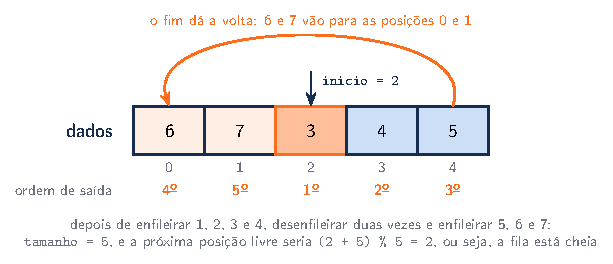
\includegraphics[width=0.85\linewidth,keepaspectratio]{imagens/capitulo-11_fila.pdf}
\end{center}

\begin{codigo}
\begin{Verbatim}[breaklines=true, breaksymbolleft={}, fontsize=\footnotesize]
#include <iostream>
using namespace std;

const int MAX = 5;             // pequeno, para ver a volta

struct Fila {
    int dados[MAX];
    int inicio = 0;            // posição do primeiro
    int tamanho = 0;           // quantos elementos há
};

bool enfileirar(Fila &f, int x) {
    if (f.tamanho == MAX) return false;        // fila cheia
    int fim = (f.inicio + f.tamanho) % MAX;    // dá a volta
    f.dados[fim] = x;
    f.tamanho++;
    return true;
}

int desenfileirar(Fila &f) {   // só se não estiver vazia
    int x = f.dados[f.inicio];
    f.inicio = (f.inicio + 1) % MAX;
    f.tamanho--;
    return x;
}

int main() {
    Fila f;
    for (int x = 1; x <= 4; x++) enfileirar(f, x);   // 1 2 3 4
    int a = desenfileirar(f);
    int b = desenfileirar(f);
    cout << a << " " << b << endl;                   // 1 2
    for (int x = 5; x <= 7; x++) enfileirar(f, x);   // 6 e 7 dão
    while (f.tamanho > 0) {                          // a volta
        cout << desenfileirar(f) << " ";
    }
    cout << endl;                                    // 3 4 5 6 7
    return 0;
}
\end{Verbatim}
\end{codigo}

Depois das duas primeiras saídas, as posições 0 e 1 do vetor ficam livres. O 5 ocupa a última posição, a 4, e o 6 e o 7 dão a volta e ocupam as posições 0 e 1. Mesmo assim, eles saem na ordem certa, porque o \texttt{inicio} também anda em círculo.

\subsection{11.6 Ponteiros e memória dinâmica}

Pilhas e filas feitas com vetores têm um limite: a capacidade \texttt{MAX}, decidida antes de o programa rodar. Para estruturas que crescem e encolhem livremente, é preciso criar espaço na memória \textbf{durante a execução}, e para isso a linguagem C++ usa \textbf{ponteiros}.

Um \textbf{ponteiro} é uma variável que guarda um \textbf{endereço} de memória, ou seja, a localização de outra variável (Capítulo 3). O operador \texttt{\&} dá o endereço de uma variável, e o operador \texttt{*} acessa o valor que está no endereço guardado pelo ponteiro:

\begin{codigo}
\begin{Verbatim}[breaklines=true, breaksymbolleft={}, fontsize=\footnotesize]
int x = 10;
int *p = &x;           // p guarda o endereço de x
cout << *p << endl;    // 10: o valor que está nesse endereço
*p = 20;               // altera x através de p
cout << x << endl;     // 20

int *q = new int(5);   // cria um int durante a execução
cout << *q << endl;    // 5
delete q;              // devolve a memória ao sistema
q = nullptr;           // agora q não aponta para nada
\end{Verbatim}
\end{codigo}

O operador \texttt{new} reserva memória para um valor e devolve o endereço dela. Essa memória não some no fim do bloco, como uma variável local: ela fica reservada até o programa a devolver com \texttt{delete}. Esquecer o \texttt{delete} causa um \textbf{vazamento de memória}: a memória fica ocupada sem uso, e um programa que roda por muito tempo pode esgotá-la. Usar um ponteiro depois do \texttt{delete} é ainda pior, porque o endereço pode já pertencer a outra coisa. O valor especial \texttt{nullptr} indica um ponteiro que não aponta para nada, e é a forma segura de marcar ``nenhum''.

Os ponteiros são uma das partes mais delicadas do C++, e a programação moderna nessa linguagem procura usá-los o mínimo possível, preferindo \texttt{vector}, \texttt{string} e as estruturas da biblioteca, que cuidam da memória sozinhas. Mas eles são a melhor forma de entender como as estruturas encadeadas funcionam por dentro.

\subsection{11.7 Lista encadeada}

Em uma \textbf{lista encadeada}, cada elemento fica em um \textbf{nó}, um registro criado com \texttt{new} que guarda o valor e um ponteiro para o \textbf{próximo} nó. Os nós podem estar em qualquer lugar da memória: o que os une é a corrente de ponteiros. A lista em si é só um ponteiro para o primeiro nó, e o último nó aponta para \texttt{nullptr}.

\begin{center}
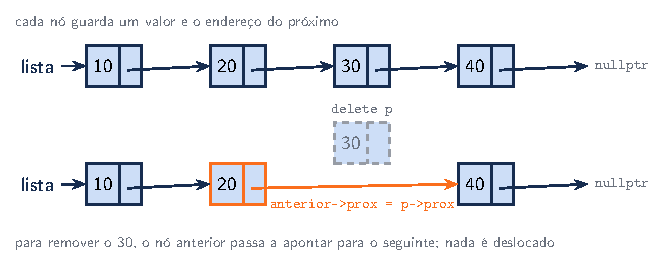
\includegraphics[width=0.9\linewidth,keepaspectratio]{imagens/capitulo-11_lista.pdf}
\end{center}

A grande vantagem da lista é que inserir e remover não exige deslocar nada: basta \textbf{religar os ponteiros}. Para inserir no início, o novo nó aponta para o antigo primeiro e passa a ser o primeiro. Para remover um nó, o anterior passa a apontar para o seguinte, e o nó removido é devolvido com \texttt{delete}. A desvantagem é que não há acesso direto: para chegar ao quinto elemento, é preciso passar pelos quatro primeiros.

\begin{codigo}
\begin{Verbatim}[breaklines=true, breaksymbolleft={}, fontsize=\footnotesize]
#include <iostream>
using namespace std;

struct No {
    int valor;
    No *prox;                  // o próximo nó (nullptr no último)
};

void inserirNoInicio(No *&lista, int x) {
    No *novo = new No;
    novo->valor = x;
    novo->prox = lista;        // aponta para o antigo primeiro
    lista = novo;              // e passa a ser o primeiro
}

void mostrar(const No *lista) {
    for (const No *p = lista; p != nullptr; p = p->prox) {
        cout << p->valor << " -> ";
    }
    cout << "fim" << endl;
}

bool remover(No *&lista, int x) {
    No *anterior = nullptr;
    No *p = lista;
    while (p != nullptr && p->valor != x) {   // procura x
        anterior = p;
        p = p->prox;
    }
    if (p == nullptr) return false;           // não achou
    if (anterior == nullptr) lista = p->prox; // era o primeiro
    else anterior->prox = p->prox;            // pula o nó
    delete p;
    return true;
}

void liberar(No *&lista) {
    while (lista != nullptr) {
        No *p = lista;
        lista = lista->prox;
        delete p;
    }
}

int main() {
    No *lista = nullptr;                      // lista vazia
    int valores[] = {40, 30, 20, 10};
    for (int x : valores) inserirNoInicio(lista, x);
    mostrar(lista);              // 10 -> 20 -> 30 -> 40 -> fim
    remover(lista, 30);
    mostrar(lista);              // 10 -> 20 -> 40 -> fim
    liberar(lista);              // devolve todos os nós
    return 0;
}
\end{Verbatim}
\end{codigo}

Três detalhes de sintaxe aparecem aqui. A seta \texttt{p->valor} é a forma curta de \texttt{(*p).valor}: o campo \texttt{valor} do nó para onde \texttt{p} aponta. O parâmetro \texttt{No *\&lista} é uma \textbf{referência para um ponteiro}: \texttt{inserirNoInicio} e \texttt{remover} precisam mudar \textbf{qual} é o primeiro nó, e por isso alteram o próprio ponteiro de quem chamou. E a função \texttt{liberar} percorre a lista devolvendo cada nó, porque todo \texttt{new} precisa de um \texttt{delete}.

\subsection{11.8 As estruturas da biblioteca}

Implementar pilhas, filas e listas é o melhor jeito de entendê-las, mas em programas reais usam-se as versões prontas da biblioteca padrão do C++, testadas e eficientes, que cuidam da memória sozinhas: \texttt{stack} (pilha), \texttt{queue} (fila), \texttt{list} (lista duplamente encadeada) e o já conhecido \texttt{vector}.

\begin{codigo}
\begin{Verbatim}[breaklines=true, breaksymbolleft={}, fontsize=\footnotesize]
#include <iostream>
#include <string>
#include <stack>
#include <queue>
using namespace std;

int main() {
    stack<int> pilha;
    pilha.push(1);
    pilha.push(2);
    pilha.push(3);
    cout << pilha.top() << endl;       // 3: o último que entrou
    pilha.pop();                       // remove o 3
    cout << pilha.top() << " " << pilha.size() << endl;   // 2 2

    queue<string> fila;
    fila.push("Ana");
    fila.push("Bruno");
    cout << fila.front() << endl;      // Ana: a primeira
    fila.pop();
    cout << fila.front() << " " << fila.empty() << endl;
    return 0;                          // Bruno 0
}
\end{Verbatim}
\end{codigo}

Repare que \texttt{pop} remove o elemento, mas não o devolve: para ler e remover, consulta-se antes com \texttt{top} (na pilha) ou \texttt{front} (na fila). A tabela resume quando usar cada estrutura:

\begin{center}
\begin{tabular}{@{}p{0.17\linewidth}p{0.36\linewidth}p{0.35\linewidth}@{}}
\toprule
\rowcolor{headergray}
\tblheader{Estrutura} & \tblheader{Faz bem} & \tblheader{Faz mal} \\
\midrule
\texttt{vector} & acesso por posição; inserir e remover no fim & inserir e remover no início ou no meio \\
\rowcolor{rowgray} \texttt{list} & inserir e remover em qualquer ponto já localizado & acesso por posição (precisa percorrer) \\
\texttt{stack} & último a entrar, primeiro a sair & qualquer acesso que não seja o topo \\
\rowcolor{rowgray} \texttt{queue} & primeiro a entrar, primeiro a sair & qualquer acesso que não seja as pontas \\
\bottomrule
\end{tabular}
\end{center}

Árvores, tabelas hash, grafos e outras estruturas, com a análise detalhada do custo de cada operação, são o assunto de um estudo próprio de estruturas de dados.

\subsection{11.9 Um programa completo: parênteses balanceados}

Compiladores, editores de código e calculadoras precisam verificar se os parênteses, colchetes e chaves de uma expressão estão \textbf{balanceados}: cada um que abre precisa ser fechado, pelo símbolo correspondente e na ordem certa. \texttt{\{a[i] * (b + c)\}} está correto; \texttt{(a + b]} e \texttt{(a + [b) - c]} não estão.

A pilha resolve o problema com elegância, porque o último símbolo aberto é sempre o primeiro que precisa ser fechado. Percorre-se a expressão: cada símbolo que abre é empilhado; cada símbolo que fecha precisa corresponder ao que está no topo, que é desempilhado. No fim, a pilha precisa estar vazia, senão sobrou algo aberto.

\begin{codigo}
\begin{Verbatim}[breaklines=true, breaksymbolleft={}, fontsize=\footnotesize]
#include <iostream>
#include <string>
#include <stack>
using namespace std;

// o símbolo que abre o par de quem fecha
char abertura(char fecha) {
    if (fecha == ')') return '(';
    if (fecha == ']') return '[';
    return '{';
}

bool balanceado(const string &expr) {
    stack<char> pilha;
    for (char c : expr) {
        if (c == '(' || c == '[' || c == '{') {
            pilha.push(c);                        // abre: guarda
        } else if (c == ')' || c == ']' || c == '}') {
            if (pilha.empty()) return false;  // fecha sem abrir
            if (pilha.top() != abertura(c)) {
                return false;                 // par trocado
            }
            pilha.pop();                          // par completo
        }
    }
    return pilha.empty();                     // sobrou aberto?
}

int main() {
    string testes[] = {"{a[i] * (b + c)}", "(a + b]",
                       "(a + [b) - c]", "((x)", "x) + (y"};
    for (const string &t : testes) {
        cout << t << ": " << (balanceado(t) ? "ok" : "erro")
             << endl;
    }
    string expr;
    cout << "Sua expressão: ";
    getline(cin, expr);
    cout << (balanceado(expr) ? "balanceada" : "não balanceada")
         << endl;
    return 0;
}
// {a[i] * (b + c)}: ok     (a + b]: erro     (a + [b) - c]: erro
// ((x): erro               x) + (y: erro
\end{Verbatim}
\end{codigo}

Cada um dos testes exercita um tipo de erro diferente: o par trocado (\texttt{(a + b]}), o cruzamento (\texttt{(a + [b) - c]}), o símbolo que sobra aberto (\texttt{((x)}) e o que fecha sem ter sido aberto (\texttt{x) + (y}), que tem o mesmo número de aberturas e fechamentos, mas na ordem errada. Contar os símbolos não bastaria para pegar os três últimos casos; a pilha pega todos.

\subsection{Erros Comuns}

\begin{itemize}
  \item \textbf{Esquecer o ponto e vírgula depois do \texttt{struct}.} A declaração termina com \texttt{\};}.
  \item \textbf{Passar registros grandes por valor sem necessidade.} Use \texttt{const Aluno \&a} quando a função só lê.
  \item \textbf{Desempilhar de uma pilha vazia ou desenfileirar de uma fila vazia.} Verifique antes com \texttt{vazia} ou \texttt{empty()}.
  \item \textbf{Esquecer a volta na fila circular.} Sem o \texttt{\% MAX}, os índices passam do fim do vetor.
  \item \textbf{Usar um ponteiro que não aponta para nada.} Acessar \texttt{p->valor} com \texttt{p} igual a \texttt{nullptr}, ou com \texttt{p} não inicializado, encerra o programa ou corrompe a memória.
  \item \textbf{Esquecer o \texttt{delete}.} Cada \texttt{new} precisa de um \texttt{delete}, senão há vazamento de memória.
  \item \textbf{Usar um nó depois do \texttt{delete}.} Leia o \texttt{prox} antes de apagar o nó, como em \texttt{liberar}.
  \item \textbf{Perder o início da lista.} Percorra com um ponteiro auxiliar (\texttt{p}); se o próprio \texttt{lista} andar, o começo da lista se perde.
  \item \textbf{Esperar que \texttt{pop()} devolva o elemento.} Nas estruturas da biblioteca, leia com \texttt{top()} ou \texttt{front()} e depois remova com \texttt{pop()}.
\end{itemize}
